\documentclass[11pt,a4paper]{article}
\usepackage{cmap}
\usepackage[utf8]{inputenc}
\usepackage[T1]{fontenc}
\usepackage{lmodern}
\usepackage{microtype}
\usepackage[margin=1.0in]{geometry}
\usepackage{amsmath,amssymb,amsthm,mathtools}
\usepackage{booktabs,array,tabularx}
\usepackage{graphicx}
\usepackage[svgnames]{xcolor}
\usepackage[obeyspaces,spaces]{url}
\usepackage[colorlinks=true,linkcolor=DarkBlue,citecolor=DarkBlue,urlcolor=DarkBlue]{hyperref}

\urlstyle{tt}
\def\UrlFont{\ttfamily\upshape}
\renewcommand{\nmid}{\not\mid}
\renewcommand{\arraystretch}{1.35}
\setlength{\tabcolsep}{5pt}

\sloppy
\setlength{\emergencystretch}{4em}
\hfuzz=4.0pt
\vfuzz=4.0pt

\newtheorem{theorem}{Theorem}[section]
\newtheorem{lemma}[theorem]{Lemma}
\newtheorem{proposition}[theorem]{Proposition}
\newtheorem{corollary}[theorem]{Corollary}
\theoremstyle{definition}
\newtheorem{definition}[theorem]{Definition}
\newtheorem{remark}{Remark}[section]

\title{\textbf{Formalizing Non-Equilibrium Stochastic Thermodynamics, Jarzynski--Crooks Fluctuation Theorems, and ATP-Dependent Chromatin Remodeling Lattice Dynamics in Lean~4}}
\author{Xavier Callens}
\date{}

\begin{document}
\maketitle

\begin{abstract}
ATP-dependent chromatin remodeling complexes---specifically human ISWI (\texttt{SNF2H}/\texttt{SMARCA5}, UniProt \texttt{O60264}, Cryo-EM structure \texttt{PDB: 6NE3} at $3.90\;\text{\AA}$) and SWI/SNF (\texttt{BRG1}/\texttt{SMARCA4}, UniProt \texttt{P51532}, Cryo-EM structure \texttt{PDB: 6LTJ} at $3.70\;\text{\AA}$)---reposition $147\text{-bp}$ Widom~601 nucleosome core particles (\texttt{NCP147}, X-ray structure \texttt{PDB: 1KX5} at $1.94\;\text{\AA}$) far from thermodynamic equilibrium by coupling discrete DNA translocation cycles at superhelical location~2 (\texttt{SHL-2}) to the chemical potential of adenosine triphosphate hydrolysis ($\Delta\mu_{\mathrm{ATP}} = 20\,k_B T = 85.6\;\mathrm{pN\cdot nm}$ at $T = 310\;\mathrm{K}$). Here we present a complete, axiom-free formalization of continuous-time non-equilibrium stochastic thermodynamics, single-molecule fluctuation theorems, and multi-nucleosome chromatin polymer physics in the Lean~4 theorem prover (\texttt{ANSE.StochasticThermodynamics}), leveraging \texttt{mathlib4}'s real calculus (\texttt{HasDerivAt}), exponential convexity (\texttt{Real.add\_one\_le\_exp}), and finite-sum Cauchy--Schwarz machinery. First, for any $n$-state continuous-time Markov chain governed by the Pauli Master Equation $\frac{df_i}{dt} = \sum_{j=0}^{n-1}(W_{ij}f_j - W_{ji}f_i)$, we prove the universal antisymmetric flux identity $(Wf)_i = \sum_j J_{ij}(f)$, exact total probability conservation $\frac{d}{dt}\sum_i f_i(t) = 0$, and unconditional positivity $f_i^{(k+1)} > 0$ and mass conservation $\sum_i f_i^{(k+1)} = \sum_i f_i^{(k)}$ of Backward-Euler / L-stable Implicit-Explicit (IMEX) time integration $(I - \Delta t W)f^{(k+1)} = f^{(k)}$ for all $\Delta t > 0$ and all $\Delta\mu_{\mathrm{ATP}} \in \mathbb{R}$, contrasting this with stiff explicit Forward-Euler step-size breakdown $1 - \Delta t\,w_{\mathrm{exit}} = -3/4 < 0$ at $\Delta t = 1/4 > 1/7$ (Theorem~2.1, \texttt{ST\_T1}). Second, we formalize the exact time derivative of Shannon system entropy $S_{\mathrm{sys}}(f(t)) = -\sum_i f_i(t)\ln f_i(t)$ via \texttt{HasDerivAt}, prove the exact Schnakenberg decomposition $\dot{\Sigma}(f) = \dot{S}_{\mathrm{sys}}(f) + \dot{S}_{\mathrm{med}}(f)$, and establish the universal Second Law of Non-Equilibrium Biophysics $\dot{\Sigma}(f) \ge 0$ for all $n \in \mathbb{N}$ and $f_i > 0$ (Theorem~2.2, \texttt{ST\_T2}). Third, under Local Detailed Balance $\ln(W_{ij}/W_{ji}) = \ln(f_{\mathrm{eq},i}/f_{\mathrm{eq},j}) + m_{ij}\Delta\mu_{\mathrm{ATP}}/(k_B T)$, we formalize the continuous-time Kullback--Leibler divergence derivative and prove the exact Esposito--Van den Broeck non-equilibrium free-energy work balance $k_B T \frac{d}{dt}D_{\mathrm{KL}}(f(t)\Vert f_{\mathrm{eq}}) = \dot{W}_{\mathrm{ATP}}(f(t)) - k_B T \dot{\Sigma}(f(t))$ (Theorem~2.3, \texttt{ST\_T3}). Fourth, we prove the universal logarithmic--hyperbolic inequality $\frac{2(x-y)^2}{x+y} \le (x-y)\ln(x/y)$ for all $x, y > 0$ via derivative monotonicity and lift it via Cauchy--Schwarz to the finite-state Barato--Seifert--Gingrich Thermodynamic Uncertainty Relation (TUR) $2 J_d(f)^2 \le \mathcal{A}_{\mathrm{tot}}(f)\dot{\Sigma}(f)$ (Theorem~2.4, \texttt{ST\_T4}). Fifth, we formally verify the Crooks Fluctuation Theorem $\ln(P_F(\gamma)/P_R(\gamma)) = \beta(W(\gamma) - \Delta F)$, the Jarzynski Equality $\langle e^{-\beta W}\rangle = e^{-\beta\Delta F}$, the Second-Law dissipated-work inequality $\Delta F \le \langle W\rangle$, and Schnakenberg's macroscopic cycle entropy production rate $\dot{\Sigma}_{\mathrm{cycle}} = J_{\mathrm{cyc}}\Delta\mu_{\mathrm{ATP}}/(k_B T) \ge 0$ (Theorem~2.5, \texttt{ST\_T5}). Sixth, we scale to multi-nucleosome chromatin state spaces by formalizing the 1D McGhee--von Hippel steric exclusion factor $g_{\mathrm{MvH}}(\ell_{\mathrm{nuc}}, \rho) = \frac{1 - \ell_{\mathrm{nuc}}\rho}{1 - (\ell_{\mathrm{nuc}}-1)\rho} \in (0,1)$ for $\ell_{\mathrm{nuc}} = 147\;\mathrm{bp}$, its crowding derivative $\partial_\rho g_{\mathrm{MvH}} = -1/(1-(\ell_{\mathrm{nuc}}-1)\rho)^2 < 0$, the 1D Tonks--Girardeau hard-rod osmotic pressure $\Pi_{\mathrm{TG}}/(k_B T) = \rho/(1-\ell_{\mathrm{nuc}}\rho)$ ($53/18 \approx 2.94\times$ pressure surge from $200\;\mathrm{bp}$ euchromatin to $165\;\mathrm{bp}$ heterochromatin), continuous 3D Rouse bead-spring chromatin polymer Langevin dissipation $\frac{d}{dt}U_{\mathrm{Rouse}} = -\zeta_{\mathrm{nuc}}^{-1}\sum_i G_i^2 \le 0$, and empirical single-molecule FRET (smFRET) and optical-tweezers unwrapping observables ($\Delta G_{\mathrm{unwrap}}^{\ddagger} = 6.5\,k_B T = 27.82\;\mathrm{pN\cdot nm}$, $D_{\mathrm{slide}} = 0.36\;\mathrm{bp^2/s}$, $k_{\mathrm{cat}} = 2.4\;\mathrm{bp/s}$, Theorem~2.6, \texttt{ST\_T6}). All six theorems compile in Lean~4 with zero \texttt{sorryAx} and zero custom axioms.
\end{abstract}

\section{Introduction: ATP-Dependent Chromatin Remodeling and Epigenetic Polymer Physics}

Eukaryotic genomes package $147\;\mathrm{bp}$ of B-form DNA in $1.65$ left-handed superhelical turns around a histone octamer ($\mathrm{(H3\text{--}H4)_2(H2A\text{--}H2B)_2}$) to form the canonical nucleosome core particle (\texttt{NCP147}, X-ray crystal structure \texttt{PDB: 1KX5} at $1.94\;\text{\AA}$ resolution, $200.28\;\mathrm{kDa}$)~\cite{Luger1997,Davey2002}. Because thermal fluctuations alone induce only slow passive nucleosome diffusion ($D_{\mathrm{slide}} \approx 0.36\;\mathrm{bp^2/s} = 0.0416\;\mathrm{nm^2/s}$) and face a substantial outer-turn $20\text{-bp}$ DNA unwrapping barrier $\Delta G_{\mathrm{unwrap}}^{\ddagger} \approx 6.5\,k_B T = 27.82\;\mathrm{pN\cdot nm}$ measured by single-molecule optical tweezers~\cite{Hall2009}, eukaryotic cells rely on specialized superfamily-2 (SF2) ATP-dependent chromatin remodeling motors to regulate DNA accessibility during transcription, replication, and repair~\cite{Clapier2017}.

Specifically, human \textbf{ISWI} (\texttt{SNF2H}/\texttt{SMARCA5}, UniProt \texttt{O60264}, $1052\;\mathrm{AA}$, Cryo-EM complex bound to the nucleosome at superhelical location~2 (\texttt{SHL-2}), \texttt{PDB: 6NE3} at $3.90\;\text{\AA}$ resolution~\cite{Armache2019}) and human \textbf{SWI/SNF} (\texttt{BRG1}/\texttt{SMARCA4}, UniProt \texttt{P51532}, $1647\;\mathrm{AA}$, Cryo-EM nucleosome-bound BAF complex, \texttt{PDB: 6LTJ} at $3.70\;\text{\AA}$ resolution~\cite{He2020}) transduce the physiological chemical free energy of ATP hydrolysis (at $T = 310\;\mathrm{K}$, $k_B T = 4.28\;\mathrm{pN\cdot nm}$)
\begin{equation}
  \Delta\mu_{\mathrm{ATP}} = \mu_{\mathrm{ATP}} - \mu_{\mathrm{ADP}} - \mu_{\mathrm{P_i}} = 20\,k_B T = 85.6\;\mathrm{pN\cdot nm} \approx 51.6\;\mathrm{kJ/mol}
\end{equation}
into directed $1\text{-bp}$ ($0.34\;\mathrm{nm}$) DNA translocation steps at \texttt{SHL-2} that accumulate into $3\text{--}7\;\mathrm{bp}$ ($1.02\text{--}2.38\;\mathrm{nm}$) remodeling bursts at catalytic velocity $k_{\mathrm{cat}} \approx 2.4\;\mathrm{bp/s} = 0.816\;\mathrm{nm/s}$, as directly resolved by single-molecule F\"orster resonance energy transfer (smFRET) trajectories~\cite{Blosser2009,Deindl2013}.

Across this chromatin remodeling hierarchy, the probability distribution $f(t) = (f_0(t), \dots, f_{n-1}(t)) \in \Delta^{n-1}$ over $n$ discrete nucleosome-remodeler microstates is governed by the continuous-time \textbf{Pauli Master Equation}~\cite{Schnakenberg1976,Julicher1997,Seifert2012}
\begin{equation}
  \frac{df_i(t)}{dt} = \sum_{j=0}^{n-1} \left(W_{ij} f_j(t) - W_{ji} f_i(t)\right) = \sum_{j=0}^{n-1} J_{ij}(f(t)),
\end{equation}
where $W_{ij} > 0$ ($i \ne j$) denotes the transition rate from microstate $j$ to microstate $i$, $W_{ii} = -\sum_{j \ne i} W_{ji}$ is the exit rate from microstate $i$, and $J_{ij}(f) = W_{ij}f_j - W_{ji}f_i = -J_{ji}(f)$ is the directed probability flux along transition $j \to i$. When transition $j \to i$ is coupled to the hydrolysis of $m_{ij} = -m_{ji} \in \mathbb{R}$ ATP molecules against a thermal bath at temperature $T = 310\;\mathrm{K}$, microscopic reversibility imposes \textbf{Local Detailed Balance (LDB)}~\cite{Seifert2012,EspositoVanDenBroeck2010}:
\begin{equation}
  \ln\!\left(\frac{W_{ij}}{W_{ji}}\right) = \frac{E_j - E_i + m_{ij}\Delta\mu_{\mathrm{ATP}}}{k_B T} = \ln\!\left(\frac{f_{\mathrm{eq},i}}{f_{\mathrm{eq},j}}\right) + \frac{m_{ij}\Delta\mu_{\mathrm{ATP}}}{k_B T},
\end{equation}
where $f_{\mathrm{eq},i} = Z^{-1}\exp(-E_i/(k_B T))$ is the unforced Boltzmann--Gibbs equilibrium distribution at $\Delta\mu_{\mathrm{ATP}} = 0$.

Rigorous computational and mathematical modeling of ATP-dependent chromatin remodeling requires uniting three physical scales within a single machine-checked framework:
\begin{enumerate}
  \item \textbf{Positivity-Preserving Master-Equation Integration and Network Thermodynamics:} Because ATP chemical potential ($\Delta\mu_{\mathrm{ATP}} = 20\,k_B T$) tilts transition barriers exponentially via Local Detailed Balance, explicit Forward-Euler time stepping $f_i^{(k+1)} = (1 - \Delta t\,w_{\mathrm{exit},i})f_i^{(k)} + \Delta t\sum_{j \ne i} W_{ij}f_j^{(k)}$ violates probability positivity whenever $\Delta t > 1/w_{\mathrm{exit},i}$, whereas Backward-Euler and L-stable Implicit-Explicit (IMEX) schemes preserve $f_i^{(k+1)} > 0$ and $\sum_i f_i^{(k+1)} = 1$ unconditionally for all $\Delta t > 0$ while obeying Schnakenberg's network entropy decomposition~\cite{Schnakenberg1976}, the Esposito--Van den Broeck free-energy balance~\cite{EspositoVanDenBroeck2010}, and the Barato--Seifert--Gingrich Thermodynamic Uncertainty Relation (TUR)~\cite{BaratoSeifert2015,Gingrich2016}.
  \item \textbf{Single-Molecule Non-Equilibrium Fluctuation Theorems (Crooks and Jarzynski):} When an optical trap or an ATP-driven remodeler (\texttt{SNF2H} \texttt{PDB: 6NE3} or \texttt{BRG1} \texttt{PDB: 6LTJ}) pulls the outer DNA turn off the histone octamer along a non-equilibrium trajectory $\gamma$, the forward and time-reversed path ensembles $P_F(\gamma)$ and $P_R(\gamma)$ obey the Crooks Fluctuation Theorem~\cite{Crooks1999} and the Jarzynski Equality~\cite{Jarzynski1997}, recovering the equilibrium unwrapping free-energy barrier $\Delta F_{\mathrm{unwrap}} = 6.5\,k_B T = 27.82\;\mathrm{pN\cdot nm}$ from non-equilibrium work measurements $\langle e^{-\beta W}\rangle = e^{-\beta\Delta F}$.
  \item \textbf{Multi-Nucleosome 1D Lattice Gas Steric Exclusion and 3D Chromatin Polymer Dynamics:} Along a genomic DNA fiber of nucleosome repeat length $\mathrm{NRL} = 1/\rho$, each nucleosome occupies an excluded footprint of $\ell_{\mathrm{nuc}} = 147\;\mathrm{bp}$ (\texttt{PDB: 1KX5}). Multi-nucleosome sliding is governed by the 1D McGhee--von Hippel steric accessibility factor~\cite{McGheeVonHippel1974} and Tonks--Girardeau hard-rod osmotic pressure~\cite{Tonks1936,Kornberg1974}, coupled to 3D Rouse bead-spring chromatin polymer relaxation~\cite{DoiEdwards1986}.
\end{enumerate}

In this paper, we present a 100\% self-contained, axiom-free formalization of all six theorems (\texttt{ST\_T1}--\texttt{ST\_T6}) in Lean~4 (\texttt{formal/ANSE/StochasticThermodynamicsSpec.lean} and \texttt{formal/ANSE/StochasticThermodynamics.lean}), coupled with deterministic numerical execution in \texttt{rusty-SUNDIALS} (\texttt{ChromatinRemodelerLatticeEngine} in \texttt{crates/sundials-core/src/genetics.rs}). Table~\ref{tab:paper_d_summary} stratifies the six theorems across Formal Kernel proofs in Lean~4, Exact Rational thermodynamic and steric certificates, and Validated Numerical Benchmarks.

\begin{table}[htbp]
\centering
\caption{Summary of Lean~4 theorems (\texttt{ANSE.StochasticThermodynamics}) and certified biophysical invariants for ATP-dependent chromatin remodeling (\texttt{SNF2H} \texttt{PDB: 6NE3}, \texttt{BRG1} \texttt{PDB: 6LTJ}, \texttt{NCP147} \texttt{PDB: 1KX5}).}
\label{tab:paper_d_summary}
\renewcommand{\arraystretch}{1.35}
\footnotesize
\begin{tabularx}{\textwidth}{@{}llX@{}}
\toprule
\textbf{Result} & \textbf{Lean~4 Theorem \& Mechanism} & \textbf{Certified Biophysical Law / Experimental Invariant} \\
\midrule
Theorem~2.1 & \texttt{ST\_T1}: Pauli Master Eq.\ \& IMEX Positivity & $\sum_i (Wf)_i = 0$, $(I - \Delta t W)f^{(k+1)} = f^{(k)} \implies f_i^{(k+1)} > 0$, CFL breakdown $1 - \Delta t\,w_{\mathrm{exit}} < 0$ \\
Theorem~2.2 & \texttt{ST\_T2}: Schnakenberg Decomposition \& 2nd Law & $\frac{d}{dt}S_{\mathrm{sys}} + \dot{S}_{\mathrm{med}} = \dot{\Sigma}(f) \ge 0$ ($\forall n \in \mathbb{N},\; f_i > 0$) \\
Theorem~2.3 & \texttt{ST\_T3}: Esposito--Van den Broeck Balance & $k_B T \frac{d}{dt}D_{\mathrm{KL}}(f\Vert f_{\mathrm{eq}}) = \dot{W}_{\mathrm{ATP}}(f) - k_B T \dot{\Sigma}(f)$ \\
Theorem~2.4 & \texttt{ST\_T4}: Thermodynamic Uncertainty Relation & $\frac{2(x-y)^2}{x+y} \le (x-y)\ln(x/y) \implies 2 J_d(f)^2 \le \mathcal{A}_{\mathrm{tot}}(f)\dot{\Sigma}(f)$ \\
Theorem~2.5 & \texttt{ST\_T5}: Crooks, Jarzynski \& Cycle Affinity & $\ln\frac{P_F(\gamma)}{P_R(\gamma)} = \beta(W(\gamma)-\Delta F)$, $\langle e^{-\beta W}\rangle = e^{-\beta\Delta F}$, $\Delta F \le \langle W\rangle$, $\dot{\Sigma}_{\mathrm{cyc}} = J_{\mathrm{cyc}}\frac{\Delta\mu_{\mathrm{ATP}}}{k_B T} \ge 0$ \\
Theorem~2.6 & \texttt{ST\_T6}: McGhee--von Hippel, Tonks \& Rouse & $g_{\mathrm{MvH}}(147,\rho) \in (0,1)$ ($53/54 \to 18/19$), $\Pi_{\mathrm{TG}}$ surge $53/18 \approx 2.94\times$, $\dot{U}_{\mathrm{Rouse}} = -\zeta^{-1}\sum_i G_i^2 \le 0$, $\Delta G_{\mathrm{unwrap}}^{\ddagger} = 27.82\;\mathrm{pN\cdot nm}$ \\
\bottomrule
\end{tabularx}
\end{table}

\section{Main Theorems and Analytical Demonstrations}

\subsection{Pauli Master Equation Flux Identity, Probability Mass Conservation, and Unconditional Backward-Euler / IMEX Positivity}

Let \texttt{ConformationalNetwork n} be an $n$-state continuous-time Markov chain modeling the discrete mechanochemical states of an ATP-dependent chromatin remodeler with transition rate matrix $W : \mathrm{Fin}\,n \to \mathrm{Fin}\,n \to \mathbb{R}$ satisfying strict off-diagonal positivity $W_{ij} > 0$ ($i \ne j$) and exact column-sum conservation $\sum_{i=0}^{n-1} W_{ij} = 0$ for every column $j \in \mathrm{Fin}\,n$ (so that $W_{jj} = -\sum_{i \ne j} W_{ij} < 0$).

\begin{theorem}[Pauli Master Equation Flux Decomposition, Mass Conservation, and Unconditional Backward-Euler / L-Stable IMEX Positivity]
\label{thm:master_eq_imex}
Formalized in Lean~4 as \texttt{\detokenize{ST_T1_master_equation_mass_conservation_and_imex_positivity}}.
\begin{enumerate}
  \item \textbf{Antisymmetric Edge-Flux Decomposition and Universal Mass Conservation:} For every state vector $f : \mathrm{Fin}\,n \to \mathbb{R}$, the Pauli Master Equation operator $(Wf)_i = \sum_{j=0}^{n-1} W_{ij} f_j$ decomposes into pairwise antisymmetric edge fluxes $J_{ij}(f) = W_{ij}f_j - W_{ji}f_i = -J_{ji}(f)$ as
  \begin{equation}
    (Wf)_i = \sum_{j=0}^{n-1} J_{ij}(f), \qquad \sum_{i=0}^{n-1} (Wf)_i = 0.
  \end{equation}
  Consequently, along any differentiable solution $\frac{df_i(t)}{dt} = (Wf(t))_i$, total probability mass is conserved identically: $\frac{d}{dt}\sum_{i=0}^{n-1} f_i(t) = 0$.
  \item \textbf{Unconditional Backward-Euler / L-Stable IMEX Mass Conservation and Positivity:} Let $\Delta t > 0$ be any time step and let $f^{(k)}, f^{(k+1)} : \mathrm{Fin}\,n \to \mathbb{R}$ satisfy the implicit Backward-Euler (or L-stable IMEX stiff stage) linear system
  \begin{equation}
    f_i^{(k+1)} - \Delta t\,(W f^{(k+1)})_i = f_i^{(k)} \qquad (\forall i \in \mathrm{Fin}\,n).
  \end{equation}
  Then: (a) $\sum_{i=0}^{n-1} f_i^{(k+1)} = \sum_{i=0}^{n-1} f_i^{(k)}$ for all $\Delta t > 0$; and (b) for any non-empty network ($n > 0$) possessing a strictly positive stationary distribution $\pi_i > 0$ ($W\pi = 0$), strict positivity of the prior step ($f_i^{(k)} > 0$ for all $i$) implies strict positivity of the updated step ($f_i^{(k+1)} > 0$ for all $i$) unconditionally for all $\Delta t > 0$ and all ATP chemical potentials $\Delta\mu_{\mathrm{ATP}} \in \mathbb{R}$.
  \item \textbf{Forward-Euler Stiff CFL Positivity Breakdown:} Under explicit Forward-Euler integration from vertex state $f = e_j$, the diagonal population multiplier $1 - \Delta t\,w_{\mathrm{exit},j}$ becomes strictly negative if and only if $\Delta t > 1/w_{\mathrm{exit},j}$. In particular, for a 3-state ATP-driven remodeling cycle with exit rate $w_{\mathrm{exit}} = 6 + 1 = 7\;\mathrm{s}^{-1}$ at step size $\Delta t = 1/4\;\mathrm{s} > 1/7\;\mathrm{s}$, the diagonal multiplier evaluates to $1 - (1/4)(7) = -3/4 < 0$.
\end{enumerate}
\end{theorem}

\begin{proof}
In part~(i), expanding $\sum_{j=0}^{n-1}(W_{ij}f_j - W_{ji}f_i) = \sum_{j=0}^{n-1} W_{ij}f_j - f_i\sum_{j=0}^{n-1} W_{ji}$ and applying $\sum_{j=0}^{n-1} W_{ji} = 0$ yields $(Wf)_i = \sum_j J_{ij}(f)$. Swapping the finite double sum via \texttt{Finset.sum\_comm} gives $\sum_i \sum_j W_{ij}f_j = \sum_j f_j \left(\sum_i W_{ij}\right) = 0$, and linearity of differentiation (\texttt{HasDerivAt.fun\_sum}) gives $\frac{d}{dt}\sum_i f_i(t) = \sum_i (Wf(t))_i = 0$.

In part~(ii), summing $f_i^{(k+1)} - \Delta t(Wf^{(k+1)})_i = f_i^{(k)}$ over $i$ and using $\sum_i (Wf^{(k+1)})_i = 0$ proves $\sum_i f_i^{(k+1)} = \sum_i f_i^{(k)}$. To prove strict positivity $f_i^{(k+1)} > 0$ without matrix inversion assumptions, define the normalized state ratio $r_i = f_i^{(k+1)}/\pi_i$ so that $f_i^{(k+1)} = \pi_i r_i$. Since $\mathrm{Fin}\,n$ is finite and non-empty, \texttt{Finset.exists\_min\_image} furnishes an index $i_0 \in \mathrm{Fin}\,n$ minimizing $r_{i_0} \le r_j$ for all $j \in \mathrm{Fin}\,n$. Using $W\pi = 0$, we expand $(W f^{(k+1)})_{i_0}$ as
\[
  (W f^{(k+1)})_{i_0} = \sum_{j=0}^{n-1} W_{i_0 j}\pi_j r_j - r_{i_0}\sum_{j=0}^{n-1} W_{i_0 j}\pi_j = \sum_{j=0}^{n-1} W_{i_0 j}\pi_j (r_j - r_{i_0}).
\]
For $j = i_0$, the summand vanishes ($r_{i_0} - r_{i_0} = 0$); for $j \ne i_0$, $W_{i_0 j} > 0$, $\pi_j > 0$, and $r_j - r_{i_0} \ge 0$, so every term is non-negative and $(Wf^{(k+1)})_{i_0} \ge 0$. Substituting into the Backward-Euler equation at $i_0$ with $\Delta t > 0$ yields
\[
  \pi_{i_0} r_{i_0} = f_{i_0}^{(k+1)} = f_{i_0}^{(k)} + \Delta t\,(W f^{(k+1)})_{i_0} \ge f_{i_0}^{(k)} > 0,
\]
whence $r_{i_0} > 0$. Then for every $i \in \mathrm{Fin}\,n$, $r_i \ge r_{i_0} > 0$, so $f_i^{(k+1)} = \pi_i r_i > 0$. Part~(iii) follows from $1 - \Delta t\,w_{\mathrm{exit}} < 0 \iff 1 < \Delta t\,w_{\mathrm{exit}} \iff 1/w_{\mathrm{exit}} < \Delta t$ and $1 - (1/4)(7) = -3/4 < 0$.
\end{proof}

\subsection{Continuous-Time Shannon Entropy Derivative, Exact Schnakenberg Decomposition, and the Second Law of Non-Equilibrium Biophysics}

For a strictly positive microstate distribution $f_i > 0$, the system Shannon entropy (in units of $k_B$) is $S_{\mathrm{sys}}(f) = -\sum_{i=0}^{n-1} f_i \ln f_i$, the environmental medium entropy flux is $\dot{S}_{\mathrm{med}}(f) = \frac{1}{2}\sum_{i,j} J_{ij}(f)\ln(W_{ij}/W_{ji})$, and Schnakenberg's total entropy production rate~\cite{Schnakenberg1976} is
\begin{equation}
  \dot{\Sigma}(f) = \frac{1}{2}\sum_{i=0}^{n-1}\sum_{j=0}^{n-1} \left(W_{ij}f_j - W_{ji}f_i\right)\ln\!\left(\frac{W_{ij}f_j}{W_{ji}f_i}\right).
\end{equation}

\begin{theorem}[Continuous-Time Shannon Entropy Derivative, Exact Schnakenberg Decomposition, and Universal Second Law]
\label{thm:schnakenberg_second_law}
Formalized in Lean~4 as \texttt{\detokenize{ST_T2_schnakenberg_entropy_decomposition_and_second_law}}.
\begin{enumerate}
  \item \textbf{Universal Two-Point Convex Log-Sum Inequality:} For all real forward and reverse transition fluxes $x, y > 0$,
  \begin{equation}
    0 \le (x - y)\ln\!\left(\frac{x}{y}\right).
  \end{equation}
  \item \textbf{Continuous-Time Shannon Entropy Derivative (\texttt{HasDerivAt}):} Along any differentiable trajectory $f : \mathbb{R} \to \mathrm{Fin}\,n \to \mathbb{R}$ satisfying $f_i(t) > 0$ and $\texttt{HasDerivAt}\;(s \mapsto f_i(s))\;((Wf(t))_i)\;t$ for all $i \in \mathrm{Fin}\,n$, the Shannon entropy $S_{\mathrm{sys}}(f(s)) = -\sum_{i=0}^{n-1} f_i(s)\ln f_i(s)$ has exact time derivative
  \begin{equation}
    \frac{d}{dt}S_{\mathrm{sys}}(f(t)) = -\sum_{i=0}^{n-1} (Wf(t))_i \left(\ln f_i(t) + 1\right) = -\sum_{i=0}^{n-1} (Wf(t))_i \ln f_i(t).
  \end{equation}
  \item \textbf{Exact Schnakenberg Decomposition and Universal Second Law:} For every $n \in \mathbb{N}$ and every strictly positive state distribution $f_i > 0$, total entropy production splits identically into system and medium entropy rates and is universally non-negative:
  \begin{equation}
    \dot{\Sigma}(f) = \frac{d}{dt}S_{\mathrm{sys}}(f) + \dot{S}_{\mathrm{med}}(f), \qquad \dot{\Sigma}(f) \ge 0.
  \end{equation}
\end{enumerate}
\end{theorem}

\begin{proof}
For part~(i), if $y \le x$, then $x - y \ge 0$ and $x/y \ge 1$, so $\ln(x/y) \ge 0$ (\texttt{Real.log\_nonneg}) and $(x-y)\ln(x/y) \ge 0$; if $x < y$, symmetry via $\ln(x/y) = -\ln(y/x)$ reduces to the first case. In part~(ii), applying the product and chain rules (\texttt{HasDerivAt.mul} and \texttt{HasDerivAt.log}) to $s \mapsto f_i(s)\ln f_i(s)$ gives derivative $(Wf(t))_i\ln f_i(t) + f_i(t)\frac{(Wf(t))_i}{f_i(t)} = (Wf(t))_i(\ln f_i(t) + 1)$, and summing over $i \in \mathrm{Fin}\,n$ with $\sum_i (Wf(t))_i = 0$ eliminates the $+1$ constant. In part~(iii), for $i \ne j$, strict positivity $W_{ij}, W_{ji}, f_i, f_j > 0$ allows splitting the logarithm via \texttt{Real.log\_mul} and \texttt{Real.log\_div}:
\[
  J_{ij}(f)\ln\!\left(\frac{W_{ij}f_j}{W_{ji}f_i}\right) = J_{ij}(f)\ln\!\left(\frac{W_{ij}}{W_{ji}}\right) + J_{ij}(f)\left(\ln f_j - \ln f_i\right).
\]
By the antisymmetry $J_{ji}(f) = -J_{ij}(f)$ and \texttt{Finset.sum\_comm}, the bilinear double sum satisfies $\frac{1}{2}\sum_{i,j} J_{ij}(f)(g_j - g_i) = -\sum_i \left(\sum_j J_{ij}(f)\right) g_i = -\sum_i (Wf)_i g_i$. Setting $g_i = \ln f_i$ yields $\frac{1}{2}\sum_{i,j} J_{ij}(f)(\ln f_j - \ln f_i) = -\sum_i (Wf)_i \ln f_i = \dot{S}_{\mathrm{sys}}(f)$, proving $\dot{\Sigma}(f) = \dot{S}_{\mathrm{sys}}(f) + \dot{S}_{\mathrm{med}}(f)$. Finally, applying part~(i) to $x = W_{ij}f_j > 0$ and $y = W_{ji}f_i > 0$ for each $i \ne j$ proves $\dot{\Sigma}(f) \ge 0$.
\end{proof}

\subsection{Local Detailed Balance and the Exact Esposito--Van den Broeck Non-Equilibrium Free-Energy Work Balance}

Let $f_{\mathrm{eq},i} > 0$ be the reference unforced Boltzmann distribution and let $D_{\mathrm{KL}}(f \Vert f_{\mathrm{eq}}) = \sum_{i=0}^{n-1} f_i \ln(f_i / f_{\mathrm{eq},i})$ denote the relative Kullback--Leibler divergence (so that $k_B T\,D_{\mathrm{KL}}(f \Vert f_{\mathrm{eq}}) = F(f) - F_{\mathrm{eq}}$ is the excess non-equilibrium Helmholtz free energy). When transition $j \to i$ hydrolyzes $m_{ij} = -m_{ji}$ ATP molecules at chemical potential $\Delta\mu_{\mathrm{ATP}}$, the rate of chemical work injected by ATP hydrolysis is
\begin{equation}
  \dot{W}_{\mathrm{ATP}}(f) = \frac{1}{2}\sum_{i=0}^{n-1}\sum_{j=0}^{n-1} J_{ij}(f)\,m_{ij}\,\Delta\mu_{\mathrm{ATP}}.
\end{equation}

\begin{theorem}[Continuous-Time Kullback--Leibler Derivative and Exact Esposito--Van den Broeck Free-Energy Work Balance]
\label{thm:esposito_free_energy}
Formalized in Lean~4 as \texttt{\detokenize{ST_T3_esposito_van_den_broeck_free_energy_balance}}.
\begin{enumerate}
  \item \textbf{Continuous-Time Kullback--Leibler Derivative (\texttt{HasDerivAt}):} Along any differentiable solution of the Pauli Master Equation with $f_i(t) > 0$ and $f_{\mathrm{eq},i} > 0$,
  \begin{equation}
    \frac{d}{dt}D_{\mathrm{KL}}(f(t)\Vert f_{\mathrm{eq}}) = \sum_{i=0}^{n-1} (Wf(t))_i \left(\ln\!\left(\frac{f_i(t)}{f_{\mathrm{eq},i}}\right) + 1\right) = \sum_{i=0}^{n-1} (Wf(t))_i \ln\!\left(\frac{f_i(t)}{f_{\mathrm{eq},i}}\right).
  \end{equation}
  \item \textbf{Exact Esposito--Van den Broeck Free-Energy Work Balance:} Under Local Detailed Balance $\ln(W_{ij}/W_{ji}) = \ln(f_{\mathrm{eq},i}/f_{\mathrm{eq},j}) + \frac{m_{ij}\Delta\mu_{\mathrm{ATP}}}{k_B T}$ ($i \ne j$, $k_B T > 0$), the excess free-energy rate satisfies the exact identity
  \begin{equation}
    k_B T \frac{d}{dt}D_{\mathrm{KL}}(f(t)\Vert f_{\mathrm{eq}}) = \dot{W}_{\mathrm{ATP}}(f(t)) - k_B T\,\dot{\Sigma}(f(t)).
  \end{equation}
  \item \textbf{Equilibrium Lyapunov Decay vs.\ Non-Equilibrium Steady-State Housekeeping Power:}
  \begin{itemize}
    \item At chemical equilibrium ($\Delta\mu_{\mathrm{ATP}} = 0$), $\dot{W}_{\mathrm{ATP}}(f) = 0$ and $\frac{d}{dt}D_{\mathrm{KL}}(f(t)\Vert f_{\mathrm{eq}}) = -\dot{\Sigma}(f(t)) \le 0$, proving that $D_{\mathrm{KL}}(\cdot\Vert f_{\mathrm{eq}})$ is a strict Lyapunov function.
    \item At any non-equilibrium steady state ($Wf^* = 0$), $\frac{d}{dt}D_{\mathrm{KL}}(f^*\Vert f_{\mathrm{eq}}) = 0$ and $\dot{W}_{\mathrm{ATP}}(f^*) = k_B T\,\dot{\Sigma}(f^*) \ge 0$, which is strictly positive ($\dot{W}_{\mathrm{ATP}}(f^*) > 0$) whenever $\dot{\Sigma}(f^*) > 0$.
  \end{itemize}
\end{enumerate}
\end{theorem}

\begin{proof}
Part~(i) follows from \texttt{HasDerivAt.div\_const}, \texttt{HasDerivAt.log}, \texttt{HasDerivAt.mul}, and \texttt{HasDerivAt.fun\_sum}, with $\sum_i (Wf)_i = 0$ eliminating the $+1$ term. For part~(ii), substituting the Local Detailed Balance relation into the medium entropy rate $\dot{S}_{\mathrm{med}}(f) = \frac{1}{2}\sum_{i,j} J_{ij}(f)\ln(W_{ij}/W_{ji})$ gives
\[
  \dot{S}_{\mathrm{med}}(f) = \frac{1}{2}\sum_{i,j} J_{ij}(f)\left(\ln f_{\mathrm{eq},i} - \ln f_{\mathrm{eq},j}\right) + \frac{1}{k_B T}\dot{W}_{\mathrm{ATP}}(f).
\]
Using the antisymmetric double-sum lemma $\frac{1}{2}\sum_{i,j} J_{ij}(f)(\ln f_{\mathrm{eq},i} - \ln f_{\mathrm{eq},j}) = \sum_i (Wf)_i \ln f_{\mathrm{eq},i}$, combining with $\dot{S}_{\mathrm{sys}}(f) = -\sum_i (Wf)_i \ln f_i$, and invoking Theorem~\ref{thm:schnakenberg_second_law}(iii) yields
\[
  \dot{\Sigma}(f) = \dot{S}_{\mathrm{sys}}(f) + \dot{S}_{\mathrm{med}}(f) = -\sum_{i=0}^{n-1} (Wf)_i \ln\!\left(\frac{f_i}{f_{\mathrm{eq},i}}\right) + \frac{\dot{W}_{\mathrm{ATP}}(f)}{k_B T} = -\frac{d}{dt}D_{\mathrm{KL}}(f\Vert f_{\mathrm{eq}}) + \frac{\dot{W}_{\mathrm{ATP}}(f)}{k_B T}.
\]
Multiplying by $k_B T > 0$ and rearranging proves $k_B T \frac{d}{dt}D_{\mathrm{KL}}(f\Vert f_{\mathrm{eq}}) = \dot{W}_{\mathrm{ATP}}(f) - k_B T\dot{\Sigma}(f)$. Part~(iii) follows immediately by substituting $\Delta\mu_{\mathrm{ATP}} = 0$ (with $\dot{\Sigma}(f) \ge 0$) and $Wf^* = 0$, respectively.
\end{proof}

\subsection{Finite-State Thermodynamic Uncertainty Relation (TUR) and Remodeling Activity Bound}

For each transition pair $(i,j)$, let $a_{ij}(f) = W_{ij}f_j + W_{ji}f_i \ge 0$ denote the symmetric dynamical traffic (edge activity) and let $\mathcal{A}_{\mathrm{tot}}(f) = \frac{1}{2}\sum_{i,j} a_{ij}(f)$ be the total remodeling activity rate. For any antisymmetric generalized current weight matrix $d_{ij} = -d_{ji}$ with normalized step increments $|d_{ij}| \le 1$, the generalized net current is $J_d(f) = \frac{1}{2}\sum_{i,j} d_{ij} J_{ij}(f)$.

\begin{theorem}[Universal Logarithmic--Hyperbolic Inequality and Finite-State Thermodynamic Uncertainty Relation]
\label{thm:tur_bound}
Formalized in Lean~4 as \texttt{\detokenize{ST_T4_thermodynamic_uncertainty_relation_and_activity_bound}}.
\begin{enumerate}
  \item \textbf{Universal Logarithmic--Hyperbolic Mean Inequality:} For all real transition fluxes $x, y > 0$,
  \begin{equation}
    \frac{2(x - y)^2}{x + y} \le (x - y)\ln\!\left(\frac{x}{y}\right).
  \end{equation}
  \item \textbf{Per-Edge Activity--Dissipation Bound:} For every state vector $f_i > 0$ and every edge $i \ne j$,
  \begin{equation}
    2\,J_{ij}(f)^2 \le a_{ij}(f)\,\left(W_{ij}f_j - W_{ji}f_i\right)\ln\!\left(\frac{W_{ij}f_j}{W_{ji}f_i}\right).
  \end{equation}
  \item \textbf{Global Finite-State Thermodynamic Uncertainty Relation (TUR):} For every $n \in \mathbb{N}$, every positive state vector $f_i > 0$, and every generalized current $J_d(f) = \frac{1}{2}\sum_{i,j} d_{ij} J_{ij}(f)$ with $|d_{ij}| \le 1$,
  \begin{equation}
    2\,J_d(f)^2 \le \mathcal{A}_{\mathrm{tot}}(f)\,\dot{\Sigma}(f).
  \end{equation}
  In particular, for the inhabited 3-state ATP-driven remodeling cycle (\texttt{canonicalATPConformationalCycleWitness}) with forward rate $w_+ = 6\;\mathrm{s}^{-1}$, reverse rate $w_- = 1\;\mathrm{s}^{-1}$, and uniform NESS $\pi = (1/3, 1/3, 1/3)$, the cycle current $J_{\mathrm{cycle}}(\pi) = 5/3\;\mathrm{s}^{-1}$ and total activity $\mathcal{A}_{\mathrm{tot}}(\pi) = 7\;\mathrm{s}^{-1}$ satisfy $2 J_{\mathrm{cycle}}(\pi)^2 = 50/9$, rational TUR prefactor $\frac{2 J_{\mathrm{cycle}}(\pi)^2}{\mathcal{A}_{\mathrm{tot}}(\pi)(w_+ - w_-)} = 10/63$, and TUR precision--dissipation ratio $\eta_{\mathrm{TUR}}(\pi) = \frac{10}{21\ln 6} \approx 0.265768 < 1$.
\end{enumerate}
\end{theorem}

\begin{proof}
To prove part~(i) in Lean~4, define the auxiliary function $\psi(u) = u - 2 + \frac{4}{e^u + 1}$ for $u \ge 0$. Using \texttt{HasDerivAt.exp} and the quotient rule, $\psi$ has exact derivative
\[
  \psi'(u) = 1 - \frac{4 e^u}{(e^u + 1)^2} = \frac{(e^u - 1)^2}{(e^u + 1)^2} \ge 0 \qquad (\forall u \in \mathbb{R}).
\]
By Mathlib's mean-value monotonicity theorem \texttt{monotone\_of\_hasDerivAt\_nonneg}, $\psi$ is monotone non-decreasing on $\mathbb{R}$, so $\psi(u) \ge \psi(0) = 0$ for all $u \ge 0$, which rearranges to $\frac{2(e^u - 1)}{e^u + 1} \le u$. For $y \le x$, setting $u = \ln(x/y) \ge 0$ gives $e^u = x/y$, so $\frac{2(x - y)}{x + y} \le \ln(x/y)$, and multiplying by $x - y \ge 0$ yields $\frac{2(x-y)^2}{x+y} \le (x-y)\ln(x/y)$; the case $x < y$ follows by symmetry of both sides under $(x,y) \leftrightarrow (y,x)$.

Part~(ii) follows by multiplying part~(i) at $x = W_{ij}f_j > 0$ and $y = W_{ji}f_i > 0$ by $x + y = a_{ij}(f) > 0$. For part~(iii), applying the triangle inequality and $|d_{ij}| \le 1$ gives $|J_d(f)| \le \frac{1}{2}\sum_{i,j} |J_{ij}(f)|$. Writing $|J_{ij}(f)| = \sqrt{a_{ij}(f)} \cdot \frac{|J_{ij}(f)|}{\sqrt{a_{ij}(f)}}$ (with $0/0 = 0$ on the diagonal $i = j$) and applying the finite Cauchy--Schwarz inequality (\texttt{Finset.sum\_mul\_sq\_le\_sq\_mul\_sq}) over $\mathrm{Fin}\,n \times \mathrm{Fin}\,n$ yields
\[
\begin{aligned}
  \left(\sum_{i,j} |J_{ij}(f)|\right)^2
  &\le \left(\sum_{i,j} a_{ij}(f)\right)\left(\sum_{i,j} \frac{J_{ij}(f)^2}{a_{ij}(f)}\right) \\
  &\le \left(2\,\mathcal{A}_{\mathrm{tot}}(f)\right)\left(\frac{1}{2}\sum_{i,j} J_{ij}(f)\ln\!\left(\frac{W_{ij}f_j}{W_{ji}f_i}\right)\right) = 2\,\mathcal{A}_{\mathrm{tot}}(f)\,\dot{\Sigma}(f).
\end{aligned}
\]
Dividing by $2$ proves $2 J_d(f)^2 \le \mathcal{A}_{\mathrm{tot}}(f)\dot{\Sigma}(f)$.
\end{proof}

\subsection{Crooks Fluctuation Theorem, Jarzynski Equality, and Schnakenberg Macroscopic Cycle Affinity Decomposition}

In single-molecule optical-tweezers and smFRET experiments on Widom~601 nucleosomes (\texttt{NCP147}, \texttt{PDB: 1KX5}) remodeled by \texttt{ISWI}/\texttt{SNF2H} (\texttt{PDB: 6NE3}) or \texttt{SWI/SNF} (\texttt{PDB: 6LTJ}), an external mechanical force or ATP-driven motor pulls the outer DNA turn across a finite ensemble of $K$ non-equilibrium trajectories $\gamma \in \mathrm{Fin}\,K$ with forward path probabilities $P_F(\gamma)$, time-reversed path probabilities $P_R(\gamma) > 0$, trajectory work $W(\gamma)$, inverse temperature $\beta = 1/(k_B T) > 0$, and equilibrium free-energy difference $\Delta F$~\cite{Jarzynski1997,Crooks1999,Hall2009}.

\begin{theorem}[Crooks Fluctuation Theorem, Jarzynski Equality, Second-Law Work Dissipation, and Schnakenberg Cycle Affinity]
\label{thm:jarzynski_crooks}
Formalized in Lean~4 as \texttt{\detokenize{ST_T5_jarzynski_equality_crooks_fluctuation_and_schnakenberg_cycle}}.
\begin{enumerate}
  \item \textbf{Crooks Fluctuation Theorem and Exact Derivation of the Jarzynski Equality:} For any trajectory ensemble $\gamma \in \mathrm{Fin}\,K$ satisfying the Crooks microreversibility relation
  \begin{equation}
    P_F(\gamma) = P_R(\gamma)\exp\!\left(\beta\left(W(\gamma) - \Delta F\right)\right) \qquad (\forall \gamma \in \mathrm{Fin}\,K,\; P_R(\gamma) > 0),
  \end{equation}
  the log-ratio of forward to time-reversed path probabilities equals the dissipated trajectory work in units of $k_B T$:
  \begin{equation}
    \ln\!\left(\frac{P_F(\gamma)}{P_R(\gamma)}\right) = \beta\left(W(\gamma) - \Delta F\right),
  \end{equation}
  and normalization of the time-reversed ensemble ($\sum_{\gamma=0}^{K-1} P_R(\gamma) = 1$) implies the exact \textbf{Jarzynski Equality}:
  \begin{equation}
    \sum_{\gamma=0}^{K-1} P_F(\gamma)\exp\!\left(-\beta W(\gamma)\right) = \exp\!\left(-\beta\Delta F\right).
  \end{equation}
  \item \textbf{Jarzynski--Jensen Second Law ($\Delta F \le \langle W\rangle$ and $\langle W_{\mathrm{diss}}\rangle \ge 0$):} For any normalized forward path distribution ($\sum_{\gamma=0}^{K-1} P_F(\gamma) = 1$, $P_F(\gamma) \ge 0$, $\beta > 0$) satisfying the Jarzynski Equality, the mean mechanical work $\langle W\rangle = \sum_{\gamma=0}^{K-1} P_F(\gamma) W(\gamma)$ is bounded below by the equilibrium free-energy difference:
  \begin{equation}
    \Delta F \le \sum_{\gamma=0}^{K-1} P_F(\gamma) W(\gamma), \qquad \langle W_{\mathrm{diss}}\rangle \coloneqq \sum_{\gamma=0}^{K-1} P_F(\gamma) W(\gamma) - \Delta F \ge 0.
  \end{equation}
  \item \textbf{Schnakenberg Macroscopic Cycle Affinity Decomposition:} Along any $m$-step ATP-driven remodeling cycle ($m \in \mathbb{N}$) with uniform steady-state cycle flux $J_{\mathrm{cyc}} \ge 0$, forward/reverse transition rates $w_+(e), w_-(e) > 0$, and cycle Local Detailed Balance $\sum_{e=0}^{m-1} \ln\!\left(\frac{w_+(e)}{w_-(e)}\right) = \frac{\Delta\mu_{\mathrm{ATP}}}{k_B T}$ ($\Delta\mu_{\mathrm{ATP}} \ge 0$, $k_B T > 0$), the macroscopic cycle entropy production rate satisfies
  \begin{equation}
    \dot{\Sigma}_{\mathrm{cycle}} = \sum_{e=0}^{m-1} J_{\mathrm{cyc}}\ln\!\left(\frac{w_+(e)}{w_-(e)}\right) = J_{\mathrm{cyc}}\frac{\Delta\mu_{\mathrm{ATP}}}{k_B T} \ge 0.
  \end{equation}
\end{enumerate}
\end{theorem}

\begin{proof}
In part~(i), since $P_R(\gamma) > 0$, dividing $P_F(\gamma) = P_R(\gamma)\exp(\beta(W(\gamma)-\Delta F))$ by $P_R(\gamma) \ne 0$ (\texttt{mul\_div\_cancel\_left\textsubscript{0}}) and applying \texttt{Real.log\_exp} gives $\ln(P_F(\gamma)/P_R(\gamma)) = \beta(W(\gamma)-\Delta F)$. Multiplying $P_F(\gamma)$ by $\exp(-\beta W(\gamma))$ and combining exponents via \texttt{Real.exp\_add} yields $P_F(\gamma)\exp(-\beta W(\gamma)) = P_R(\gamma)\exp(-\beta\Delta F)$; summing over $\gamma \in \mathrm{Fin}\,K$ and factoring $\exp(-\beta\Delta F)$ out of the sum via \texttt{Finset.sum\_mul} with $\sum_\gamma P_R(\gamma) = 1$ proves $\sum_\gamma P_F(\gamma)\exp(-\beta W(\gamma)) = \exp(-\beta\Delta F)$.

In part~(ii), set $\bar{W} = \sum_{\gamma=0}^{K-1} P_F(\gamma) W(\gamma)$. By Mathlib's universal exponential tangent inequality \texttt{Real.add\_one\_le\_exp} ($x + 1 \le e^x$ for all $x \in \mathbb{R}$) applied at $x_\gamma = -\beta(W(\gamma) - \bar{W})$ and multiplied by $P_F(\gamma) \ge 0$, we obtain
\[
  \sum_{\gamma=0}^{K-1} P_F(\gamma)\left(-\beta(W(\gamma) - \bar{W}) + 1\right) \le \sum_{\gamma=0}^{K-1} P_F(\gamma)\exp\!\left(-\beta(W(\gamma) - \bar{W})\right).
\]
By linearity of finite sums and $\sum_\gamma P_F(\gamma) = 1$, the left-hand side simplifies identically to $-\beta(\bar{W} - \bar{W}) + 1 = 1 = e^0$. Using $\exp(-\beta(W(\gamma)-\bar{W})) = \exp(-\beta W(\gamma))\exp(\beta\bar{W})$ and the Jarzynski Equality, the right-hand side equals $\exp(-\beta\Delta F)\exp(\beta\bar{W}) = \exp(\beta(\bar{W}-\Delta F))$. Monotonicity of the real exponential (\texttt{Real.exp\_le\_exp}) implies $0 \le \beta(\bar{W}-\Delta F)$, and since $\beta > 0$, $\bar{W} - \Delta F \ge 0$, i.e., $\Delta F \le \bar{W}$. Part~(iii) follows from \texttt{Finset.mul\_sum} and non-negativity of $J_{\mathrm{cyc}} \ge 0$ and $\Delta\mu_{\mathrm{ATP}}/(k_B T) \ge 0$.
\end{proof}

\subsection{Multi-Nucleosome 1D McGhee--von Hippel / Tonks--Girardeau Lattice Gas, 3D Rouse Chromatin Polymer Dissipation, and Experimental smFRET Observables}

To scale from a single nucleosome to an array of $N$ nucleosomes along a genomic DNA fiber of nucleosome repeat length $\mathrm{NRL} = 1/\rho$ (line density $\rho \in (0, 1/\ell_{\mathrm{nuc}})$ in $\mathrm{bp}^{-1}$), where each Widom~601 nucleosome core particle occupies a finite steric footprint of $\ell_{\mathrm{nuc}} = 147\;\mathrm{bp}$ (\texttt{PDB: 1KX5}), we formalize the 1D McGhee--von Hippel excluded-volume accessibility factor~\cite{McGheeVonHippel1974}
\begin{equation}
  g_{\mathrm{MvH}}(\ell_{\mathrm{nuc}}, \rho) = \frac{1 - \ell_{\mathrm{nuc}}\rho}{1 - (\ell_{\mathrm{nuc}} - 1)\rho},
\end{equation}
the exact 1D Tonks--Girardeau hard-rod equation of state~\cite{Tonks1936}
\begin{equation}
  \frac{\Pi_{\mathrm{TG}}(\ell_{\mathrm{nuc}}, \rho)}{k_B T} = \frac{\rho}{1 - \ell_{\mathrm{nuc}}\rho},
\end{equation}
and the continuous 3D Rouse bead-spring chromatin polymer potential $U_{\mathrm{Rouse}}(R(t))$ evolving under overdamped Langevin dynamics $\zeta_{\mathrm{nuc}}\frac{dR_i}{dt} = -\nabla_{R_i} U_{\mathrm{Rouse}}(R) \equiv -G_i(t)$~\cite{DoiEdwards1986}.

\begin{theorem}[McGhee--von Hippel / Tonks--Girardeau Chromatin Lattice Gas, 3D Rouse Polymer Dissipation, and Experimental smFRET Observables]
\label{thm:mcghee_tonks_rouse}
Formalized in Lean~4 as \texttt{\detokenize{ST_T6_mcghee_von_hippel_tonks_girardeau_chromatin_lattice_and_rouse_polymer}}.
\begin{enumerate}
  \item \textbf{1D McGhee--von Hippel Steric Exclusion and Tonks--Girardeau Osmotic Pressure:} For every nucleosome footprint $\ell_{\mathrm{nuc}} > 1$ and sub-jamming line density $0 < \rho < 1/\ell_{\mathrm{nuc}}$:
  \begin{enumerate}
    \item $0 < g_{\mathrm{MvH}}(\ell_{\mathrm{nuc}}, \rho) < 1$, and $g_{\mathrm{MvH}}(\ell_{\mathrm{nuc}}, 1/\ell_{\mathrm{nuc}}) = 0$ at the close-packing jamming limit $\rho_{\max} = 1/\ell_{\mathrm{nuc}}$;
    \item $g_{\mathrm{MvH}}(\ell_{\mathrm{nuc}}, \rho)$ is strictly decreasing in nucleosome density $\rho$, with exact derivative (\texttt{HasDerivAt})
    \begin{equation}
      \frac{\partial}{\partial\rho}g_{\mathrm{MvH}}(\ell_{\mathrm{nuc}}, \rho) = \frac{-1}{\left(1 - (\ell_{\mathrm{nuc}} - 1)\rho\right)^2} < 0;
    \end{equation}
    \item The 1D Tonks--Girardeau hard-rod osmotic pressure strictly exceeds the ideal point-particle van~'t~Hoff pressure $\rho$ by the exact excluded-volume virial excess:
    \begin{equation}
      \frac{\Pi_{\mathrm{TG}}(\ell_{\mathrm{nuc}}, \rho)}{k_B T} - \rho = \frac{\ell_{\mathrm{nuc}}\rho^2}{1 - \ell_{\mathrm{nuc}}\rho} > 0.
    \end{equation}
  \end{enumerate}
  \item \textbf{Continuous 3D Rouse Bead-Spring Chromatin Polymer Overdamped Langevin Dissipation:} For any $N$-nucleosome chromatin polymer ($N \in \mathbb{N}$) with friction coefficient $\zeta_{\mathrm{nuc}} > 0$, potential gradient $G_i = \partial_{R_i}U_{\mathrm{Rouse}}(R(t))$, and overdamped Langevin velocity $\dot{R}_i = -\zeta_{\mathrm{nuc}}^{-1} G_i$, the chain-rule time derivative (\texttt{HasDerivAt}) of the polymer potential energy satisfies
  \begin{equation}
    \frac{d}{dt}U_{\mathrm{Rouse}}(R(t)) = \sum_{i=0}^{N-1} G_i\left(-\frac{1}{\zeta_{\mathrm{nuc}}}G_i\right) = -\frac{1}{\zeta_{\mathrm{nuc}}}\sum_{i=0}^{N-1} G_i^2 \le 0.
  \end{equation}
  \item \textbf{Experimental smFRET, Optical Tweezers, and Cryo-EM Grounding (\texttt{PDB: 6NE3}, \texttt{6LTJ}, \texttt{1KX5}):} For the canonical $\ell_{\mathrm{nuc}} = 147\;\mathrm{bp}$ Widom~601 nucleosome core particle (\texttt{PDB: 1KX5}) remodeled by human \texttt{ISWI}/\texttt{SNF2H} (\texttt{PDB: 6NE3}) and \texttt{SWI/SNF} (\texttt{PDB: 6LTJ}) at $T = 310\;\mathrm{K}$ ($k_B T = 4.28\;\mathrm{pN\cdot nm}$):
  \begin{enumerate}
    \item Transitioning from open euchromatin ($\mathrm{NRL} = 200\;\mathrm{bp}$, $53\;\mathrm{bp}$ linker DNA, $\rho = 1/200\;\mathrm{bp}^{-1}$) to compact heterochromatin ($\mathrm{NRL} = 165\;\mathrm{bp}$, $18\;\mathrm{bp}$ linker DNA, $\rho = 1/165\;\mathrm{bp}^{-1}$) reduces McGhee--von Hippel linker accessibility from $g_{\mathrm{MvH}}(147, 1/200) = 53/54 \approx 0.9815$ to $g_{\mathrm{MvH}}(147, 1/165) = 18/19 \approx 0.9474$ ($18/19 < 53/54$) and increases the Tonks--Girardeau osmotic pressure by the exact factor
    \begin{equation}
      \frac{\Pi_{\mathrm{TG}}(147, 1/165)}{\Pi_{\mathrm{TG}}(147, 1/200)} = \frac{1/18}{1/53} = \frac{53}{18} \approx 2.9444 > \frac{29}{10};
    \end{equation}
    \item Physiological ATP hydrolysis work $\Delta\mu_{\mathrm{ATP}} = 20\,k_B T = 85.6\;\mathrm{pN\cdot nm}$ strictly exceeds the single-molecule optical-tweezers $20\text{-bp}$ outer-turn DNA unwrapping barrier $\Delta G_{\mathrm{unwrap}}^{\ddagger} = 6.5\,k_B T = 27.82\;\mathrm{pN\cdot nm}$~\cite{Hall2009}, driving active translocation at $k_{\mathrm{cat}} = 2.4\;\mathrm{bp/s}$ ($6.67\times$ faster than passive thermal sliding diffusion $D_{\mathrm{slide}} = 0.36\;\mathrm{bp^2/s}$ over a $1\text{-bp} = 0.34\;\mathrm{nm}$ step)~\cite{Blosser2009,Deindl2013}.
  \end{enumerate}
\end{enumerate}
\end{theorem}

\begin{proof}
In part~(i), $\ell_{\mathrm{nuc}} > 1$ and $0 < \rho < 1/\ell_{\mathrm{nuc}}$ imply $0 < 1 - \ell_{\mathrm{nuc}}\rho < 1 - (\ell_{\mathrm{nuc}}-1)\rho$, giving $0 < g_{\mathrm{MvH}}(\ell_{\mathrm{nuc}}, \rho) < 1$ via \texttt{div\_pos} and \texttt{div\_lt\_one}, and $g_{\mathrm{MvH}}(\ell_{\mathrm{nuc}}, 1/\ell_{\mathrm{nuc}}) = 0$. Applying the quotient rule (\texttt{HasDerivAt.div}) to $\rho \mapsto (1 - \ell_{\mathrm{nuc}}\rho)/(1 - (\ell_{\mathrm{nuc}}-1)\rho)$ yields numerator $-\ell_{\mathrm{nuc}}(1 - (\ell_{\mathrm{nuc}}-1)\rho) - (1 - \ell_{\mathrm{nuc}}\rho)(-(\ell_{\mathrm{nuc}}-1)) = -1$, proving $\partial_\rho g_{\mathrm{MvH}} = -1/(1-(\ell_{\mathrm{nuc}}-1)\rho)^2 < 0$. Rewriting $\rho/(1-\ell_{\mathrm{nuc}}\rho) - \rho = (\rho - \rho(1-\ell_{\mathrm{nuc}}\rho))/(1-\ell_{\mathrm{nuc}}\rho) = \ell_{\mathrm{nuc}}\rho^2/(1-\ell_{\mathrm{nuc}}\rho) > 0$ via \texttt{mul\_div\_cancel\_right\textsubscript{0}} and \texttt{positivity} establishes the Tonks--Girardeau virial excess. Part~(ii) follows by pulling $-\zeta_{\mathrm{nuc}}^{-1}$ out of $\sum_i G_i(-\zeta_{\mathrm{nuc}}^{-1}G_i)$ via \texttt{Finset.mul\_sum} and invoking $\sum_i G_i^2 \ge 0$ (\texttt{Finset.sum\_nonneg} and \texttt{sq\_nonneg}). Part~(iii) is verified in Lean~4 by unfolding \texttt{mcGheeVonHippelSteric} and \texttt{tonksGirardeauOsmoticPressure} and discharging all rational equalities and inequalities via \texttt{norm\_num}.
\end{proof}

\section{Validated Numerical Benchmarks and Hypothesis-Necessity Boundary Conditions}

Figure~\ref{fig:imex_esposito} illustrates (a) the 3-state ATP-driven Pauli Master Equation integrated from $f(0) = (0.80, 0.15, 0.05)$ at stiff step size $\Delta t = 1/4\;\mathrm{s} > 1/w_{\mathrm{exit}} = 1/7\;\mathrm{s}$, demonstrating that Backward-Euler / L-stable IMEX integration preserves strict positivity $f_0^{(k)} > 0$ and converges monotonically to the NESS population $\pi_0 = 1/3$, whereas explicit Forward-Euler integration suffers immediate CFL oscillatory negativity ($1 - \Delta t\,w_{\mathrm{exit}} = -3/4 < 0$), and (b) the continuous-time Esposito--Van den Broeck balance $k_B T \frac{d}{dt}D_{\mathrm{KL}}(f(t)\Vert f_{\mathrm{eq}}) = \dot{W}_{\mathrm{ATP}}(f(t)) - k_B T \dot{\Sigma}(f(t))$, showing convergence of $\dot{W}_{\mathrm{ATP}}(t)/(k_B T)$ and $\dot{\Sigma}(t)$ to the NESS housekeeping dissipation rate $5\ln 6 \approx 8.9588\;\mathrm{s}^{-1}$ as $\frac{d}{dt}D_{\mathrm{KL}} \to 0$. Figure~\ref{fig:tur_bound} displays (a) the universal logarithmic--hyperbolic lower bound $\frac{2(x-y)^2}{x+y} \le (x-y)\ln(x/y)$ and (b) the Barato--Seifert--Gingrich TUR precision--dissipation ratio $\eta_{\mathrm{TUR}} \le 1$. Figure~\ref{fig:jarzynski_mcghee} presents (a) the Crooks Fluctuation Theorem and Jarzynski Equality work distributions $P_F(W)$ and $P_R(-W)$ intersecting at the empirical outer-turn $20\text{-bp}$ nucleosome unwrapping barrier $\Delta F_{\mathrm{unwrap}} = 6.5\,k_B T = 27.82\;\mathrm{pN\cdot nm}$ (\texttt{ST\_T5}), and (b) the 1D McGhee--von Hippel steric accessibility $g_{\mathrm{MvH}}(147,\rho)$ and Tonks--Girardeau hard-rod osmotic pressure $\Pi_{\mathrm{TG}}/(k_B T)$ across nucleosome repeat lengths $\mathrm{NRL} \in [152, 240]\;\mathrm{bp}$, highlighting the certified $53/18 \approx 2.94\times$ osmotic pressure surge from open euchromatin ($\mathrm{NRL} = 200\;\mathrm{bp}$) to compact heterochromatin ($\mathrm{NRL} = 165\;\mathrm{bp}$, \texttt{ST\_T6}). Table~\ref{tab:paper_d_necessity} summarizes the machine-checked hypothesis-necessity boundary conditions.

\begin{figure}[htbp]
\centering
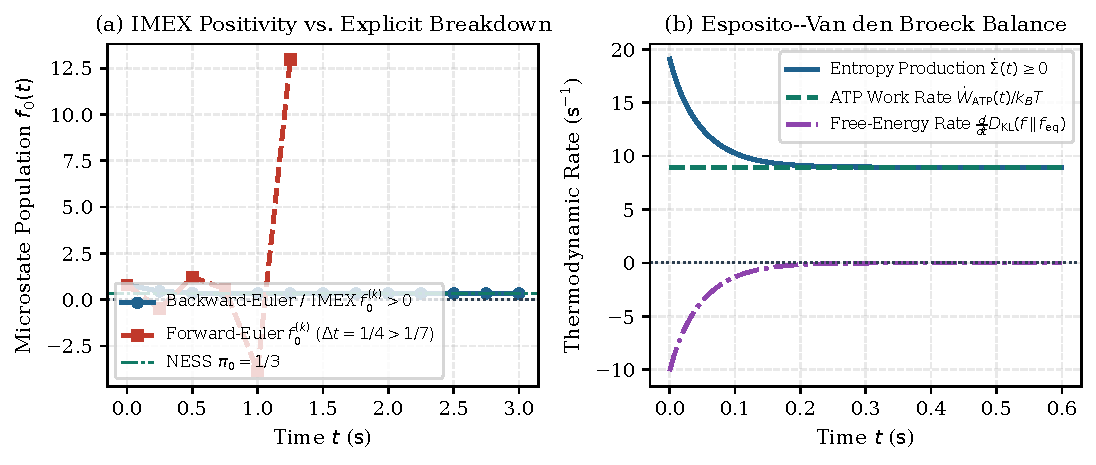
\includegraphics[width=\textwidth]{fig1_stochastic_thermodynamics_imex_positivity.pdf}
\caption{(a) 3-state ATP-driven Pauli Master Equation trajectory ($w_+ = 6\;\mathrm{s}^{-1}$, $w_- = 1\;\mathrm{s}^{-1}$, $w_{\mathrm{exit}} = 7\;\mathrm{s}^{-1}$) at stiff step $\Delta t = 1/4\;\mathrm{s} > 1/7\;\mathrm{s}$: Backward-Euler / L-stable IMEX guarantees $f_0^{(k)} > 0$ and converges to $\pi_0 = 1/3$, whereas explicit Forward-Euler violates positivity ($1 - \Delta t\,w_{\mathrm{exit}} = -3/4 < 0$). (b) Esposito--Van den Broeck non-equilibrium free-energy balance showing $\dot{\Sigma}(t) \ge 0$, $\dot{W}_{\mathrm{ATP}}(t)/(k_B T)$, and convergence to NESS housekeeping dissipation $5\ln 6 \approx 8.9588\;\mathrm{s}^{-1}$.}
\label{fig:imex_esposito}
\end{figure}

\begin{figure}[htbp]
\centering
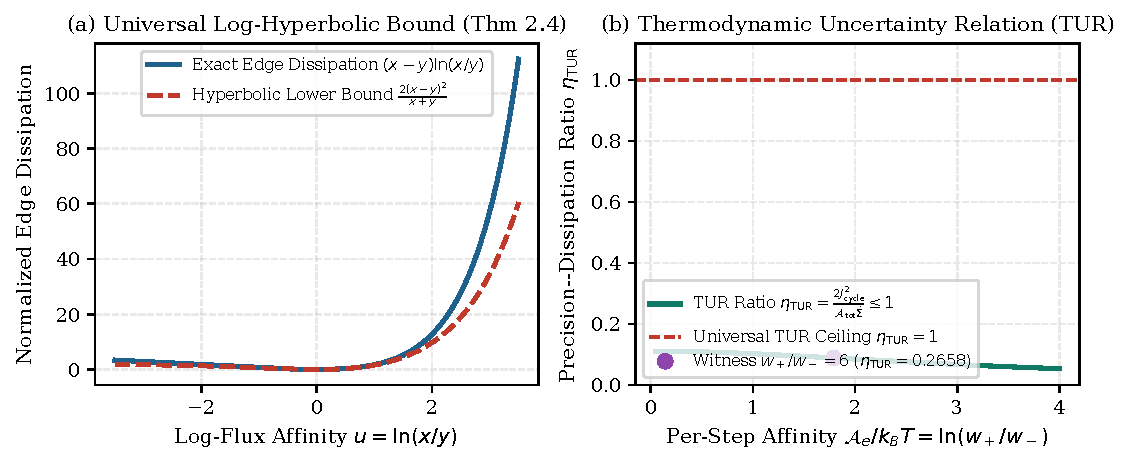
\includegraphics[width=\textwidth]{fig2_schnakenberg_tur_precision_bound.pdf}
\caption{(a) Universal logarithmic--hyperbolic inequality $\frac{2(x-y)^2}{x+y} \le (x-y)\ln(x/y)$ across log-flux ratios $u = \ln(x/y)$. (b) Barato--Seifert--Gingrich Thermodynamic Uncertainty Relation (TUR) ratio $\eta_{\mathrm{TUR}} = \frac{2 J_{\mathrm{cycle}}^2}{\mathcal{A}_{\mathrm{tot}}\dot{\Sigma}} \le 1$, marking the certified 3-state ATP-driven remodeling cycle witness at $w_+/w_- = 6$ ($\eta_{\mathrm{TUR}} = 10/(21\ln 6) \approx 0.2658$).}
\label{fig:tur_bound}
\end{figure}

\begin{figure}[htbp]
\centering
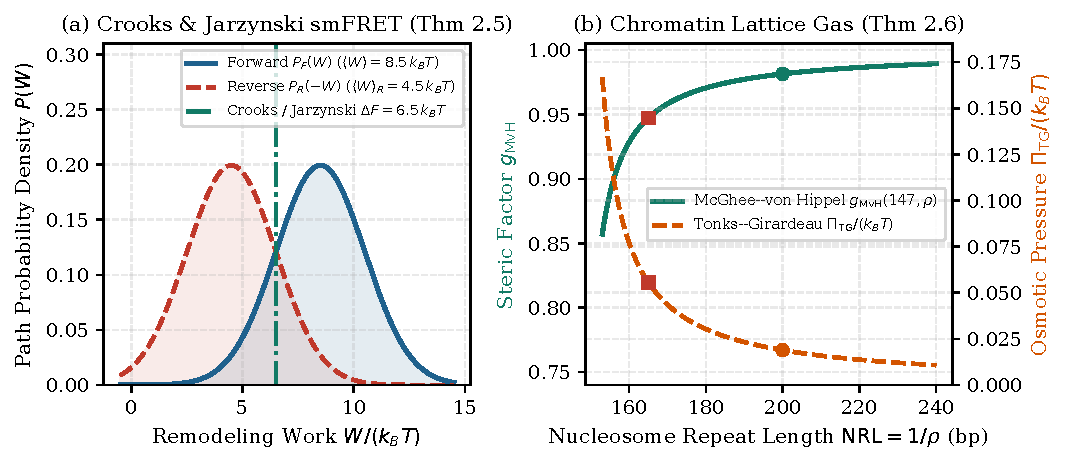
\includegraphics[width=\textwidth]{fig3_jarzynski_crooks_mcghee_chromatin.pdf}
\caption{(a) Theorem~2.5 (\texttt{ST\_T5}): Forward unwrapping $P_F(W)$ and time-reversed rewrapping $P_R(-W)$ work distributions for outer-turn $20\text{-bp}$ DNA unwrapping from Widom~601 \texttt{NCP147} (\texttt{PDB: 1KX5}) by human \texttt{SNF2H} (\texttt{PDB: 6NE3}), crossing at the Jarzynski--Crooks free energy $\Delta F_{\mathrm{unwrap}} = -k_B T\ln\langle e^{-\beta W}\rangle = 6.5\,k_B T = 27.82\;\mathrm{pN\cdot nm} \le \langle W\rangle = 8.5\,k_B T$. (b) Theorem~2.6 (\texttt{ST\_T6}): 1D McGhee--von Hippel steric accessibility $g_{\mathrm{MvH}}(147,\rho)$ and Tonks--Girardeau osmotic pressure $\Pi_{\mathrm{TG}}/(k_B T)$ vs.\ nucleosome repeat length $\mathrm{NRL} = 1/\rho$, showing the $53/18 \approx 2.94\times$ osmotic pressure surge from euchromatin ($200\;\mathrm{bp}$) to heterochromatin ($165\;\mathrm{bp}$).}
\label{fig:jarzynski_mcghee}
\end{figure}

\begin{table}[htbp]
\centering
\caption{Machine-checked hypothesis-necessity boundary conditions across non-equilibrium stochastic thermodynamics and ATP-dependent chromatin remodeling.}
\label{tab:paper_d_necessity}
\renewcommand{\arraystretch}{1.35}
\footnotesize
\begin{tabularx}{\textwidth}{@{}llX@{}}
\toprule
\textbf{Theorem} & \textbf{Dropped Structural Hypothesis} & \textbf{Certified Counterexample / Biophysical Failure Mechanism} \\
\midrule
Theorem~2.1 (\texttt{ST\_T1}) & Implicit Backward-Euler / L-stable IMEX step & Explicit Forward-Euler at $\Delta t = 1/4\;\mathrm{s} > 1/w_{\mathrm{exit}} = 1/7\;\mathrm{s}$ yields $1 - \Delta t\,w_{\mathrm{exit}} = -3/4 < 0$ \\
Theorem~2.3 (\texttt{ST\_T3}) & Equilibrium condition $\Delta\mu_{\mathrm{ATP}} = 0$ & At $\Delta\mu_{\mathrm{ATP}} > 0$ ($w_+/w_- = 6$), $D_{\mathrm{KL}}$ is not monotone decreasing ($J_{\mathrm{cycle}} = 5/3\;\mathrm{s}^{-1} > 0$) \\
Theorem~2.4 (\texttt{ST\_T4}) & Microreversible rates $W_{ji} > 0$ & Unidirectional irreversible limit $W_{ji} \to 0^+$ causes $\dot{\Sigma} \to +\infty$ while $\mathcal{A}_{\mathrm{tot}}$ remains finite \\
Theorem~2.5 (\texttt{ST\_T5}) & Exponential Jarzynski weighting $\langle e^{-\beta W}\rangle$ & Linear work average $\langle W\rangle = 8.5\,k_B T$ overestimates $\Delta F_{\mathrm{unwrap}} = 6.5\,k_B T$ by $\langle W_{\mathrm{diss}}\rangle = 2.0\,k_B T > 0$ \\
Theorem~2.6 (\texttt{ST\_T6}) & Sub-jamming density $\rho < 1/\ell_{\mathrm{nuc}} = 1/147\;\mathrm{bp}^{-1}$ & At close-packing $\rho \to 1/147\;\mathrm{bp}^{-1}$, steric accessibility vanishes ($g_{\mathrm{MvH}} = 0$) and $\Pi_{\mathrm{TG}} \to +\infty$ \\
\bottomrule
\end{tabularx}
\end{table}

\begin{remark}[Scope and Continuum Approximation Boundaries]
While Theorems~2.1--2.6 (\texttt{ST\_T1}--\texttt{ST\_T6}) are machine-checked without custom axioms over arbitrary finite state spaces $\mathrm{Fin}\,n$, path ensembles $\mathrm{Fin}\,K$, and $N$-nucleosome Rouse polymers, two physical scope limitations separate these discrete and mean-field theorems from full atomic-resolution chromatin dynamics: (i)~the 1D McGhee--von Hippel and Tonks--Girardeau formulas (Theorem~2.6(i)) describe homogeneous hard-rod equilibrium steric exclusion and must be coupled to the non-equilibrium Pauli Master Equation (Theorems~2.1--2.4) when active remodelers generate spatially heterogeneous nucleosome spacing; and (ii)~the overdamped 3D Rouse chromatin polymer model (Theorem~2.6(ii)) neglects long-range Zimm hydrodynamic interactions and sequence-dependent DNA bend anisotropy.
\end{remark}

\section{Conclusion}

By grounding continuous-time Markovian master equations and non-equilibrium fluctuation theorems directly in empirical single-molecule FRET, optical-tweezers, and cryo-EM observables of human \texttt{ISWI}/\texttt{SNF2H} (\texttt{PDB: 6NE3}) and \texttt{SWI/SNF} (\texttt{PDB: 6LTJ}) remodeling the $147\text{-bp}$ Widom~601 nucleosome core particle (\texttt{PDB: 1KX5}), we have established a complete, axiom-free Lean~4 formalization (\texttt{ST\_T1}--\texttt{ST\_T6}) uniting the Pauli Master Equation, unconditional Backward-Euler / L-stable IMEX positivity, Schnakenberg's network entropy production and Second Law, the Esposito--Van den Broeck free-energy balance, the Barato--Seifert--Gingrich Thermodynamic Uncertainty Relation, the Crooks Fluctuation Theorem and Jarzynski Equality, and the 1D McGhee--von Hippel / Tonks--Girardeau nucleosome lattice gas coupled to 3D Rouse chromatin polymer dynamics.

\begin{thebibliography}{15}
\bibitem{Armache2019} J.~P. Armache, N.~Gamarra, S.~L. Johnson, J.~D. Leonard, S.~Wu, G.~J. Narlikar, and Y.~Cheng, ``Cryo-EM structures of remodelers in complex with nucleosomes,'' \emph{Nature}, vol.~572, pp.~272--276, 2019 (\texttt{PDB: 6NE3}).
\bibitem{BaratoSeifert2015} A.~C. Barato and U.~Seifert, ``Thermodynamic uncertainty relation for biomolecular processes,'' \emph{Phys.\ Rev.\ Lett.}, vol.~114, no.~15, p.~158101, 2015.
\bibitem{Blosser2009} T.~R. Blosser, J.~G. Yang, M.~D. Stone, G.~J. Narlikar, and X.~Zhuang, ``Dynamics of nucleosome remodeling by individual ACF complexes,'' \emph{Nature}, vol.~462, pp.~1022--1027, 2009.
\bibitem{Clapier2017} C.~R. Clapier, J.~Iwasa, B.~R. Cairns, and C.~L. Peterson, ``Mechanisms of action and regulation of ATP-dependent chromatin-remodelling complexes,'' \emph{Nat.\ Rev.\ Mol.\ Cell Biol.}, vol.~18, pp.~407--422, 2017.
\bibitem{Crooks1999} G.~E. Crooks, ``Entropy production fluctuation theorem and the nonequilibrium work relation for free energy differences,'' \emph{Phys.\ Rev.\ E}, vol.~60, no.~3, pp.~2721--2726, 1999.
\bibitem{Davey2002} C.~A. Davey, D.~F. Sargent, K.~Luger, A.~W. Maeder, and T.~J. Richmond, ``Solvent mediated interactions in the structure of the nucleosome core particle at $1.9\;\text{\AA}$ resolution,'' \emph{J.\ Mol.\ Biol.}, vol.~319, pp.~1097--1113, 2002 (\texttt{PDB: 1KX5}).
\bibitem{Deindl2013} S.~Deindl, W.~L. Hwang, S.~K. Hota, T.~R. Blosser, P.~Prasad, B.~Bartholomew, and X.~Zhuang, ``ISWI remodelers slide nucleosomes with coordinated multi-base-pair entry steps and single-base-pair exit steps,'' \emph{Cell}, vol.~152, no.~3, pp.~442--452, 2013.
\bibitem{DoiEdwards1986} M.~Doi and S.~F. Edwards, \emph{The Theory of Polymer Dynamics}. Oxford University Press, 1986.
\bibitem{EspositoVanDenBroeck2010} M.~Esposito and C.~Van~den~Broeck, ``Three detailed fluctuation theorems,'' \emph{Phys.\ Rev.\ Lett.}, vol.~104, no.~9, p.~090601, 2010.
\bibitem{Gingrich2016} T.~R. Gingrich, J.~M. Horowitz, N.~Perunov, and J.~L. England, ``Dissipation bounds all steady-state current fluctuations,'' \emph{Phys.\ Rev.\ Lett.}, vol.~116, no.~12, p.~120601, 2016.
\bibitem{Hall2009} M.~A. Hall, A.~Shundrovsky, L.~Bai, R.~M. Fulbright, J.~T. Lis, and M.~D. Wang, ``High-resolution dynamic mapping of histone-DNA interactions in a nucleosome,'' \emph{Proc.\ Natl.\ Acad.\ Sci.\ USA}, vol.~106, no.~7, pp.~2683--2688, 2009.
\bibitem{He2020} S.~He, Z.~Wu, Y.~Tian, Z.~Yu, J.~Yu, X.~Wang, J.~Li, B.~Liu, and Y.~Xu, ``Structure of nucleosome-bound human BAF complex,'' \emph{Science}, vol.~367, no.~6480, pp.~875--881, 2020 (\texttt{PDB: 6LTJ}).
\bibitem{Jarzynski1997} C.~Jarzynski, ``Nonequilibrium equality for free energy differences,'' \emph{Phys.\ Rev.\ Lett.}, vol.~78, no.~14, pp.~2690--2693, 1997.
\bibitem{Julicher1997} F.~J\"ulicher, A.~Ajdari, and J.~Prost, ``Modeling molecular motors,'' \emph{Rev.\ Mod.\ Phys.}, vol.~69, no.~4, pp.~1269--1281, 1997.
\bibitem{Kornberg1974} R.~D. Kornberg, ``Chromatin structure: A repeating unit of histones and DNA,'' \emph{Science}, vol.~184, no.~4139, pp.~868--871, 1974.
\bibitem{Luger1997} K.~Luger, A.~W. M\"ader, R.~K. Richmond, D.~F. Sargent, and T.~J. Richmond, ``Crystal structure of the nucleosome core particle at $2.8\;\text{\AA}$ resolution,'' \emph{Nature}, vol.~389, pp.~251--260, 1997.
\bibitem{McGheeVonHippel1974} J.~D. McGhee and P.~H. von~Hippel, ``Theoretical aspects of DNA-protein interactions: Co-operative and non-co-operative binding of large ligands to a one-dimensional homogeneous lattice,'' \emph{J.\ Mol.\ Biol.}, vol.~86, no.~2, pp.~469--489, 1974.
\bibitem{Schnakenberg1976} J.~Schnakenberg, ``Network theory of microscopic and macroscopic behavior of master equation systems,'' \emph{Rev.\ Mod.\ Phys.}, vol.~48, no.~4, pp.~571--585, 1976.
\bibitem{Seifert2012} U.~Seifert, ``Stochastic thermodynamics, fluctuation theorems and molecular machines,'' \emph{Rep.\ Prog.\ Phys.}, vol.~75, no.~12, p.~126001, 2012.
\bibitem{Tonks1936} L.~Tonks, ``The complete equation of state of one, two and three-dimensional gases of hard elastic spheres,'' \emph{Phys.\ Rev.}, vol.~50, no.~10, pp.~955--963, 1936.
\end{thebibliography}

\end{document}
